\documentclass{article}

\usepackage{spconf,amsmath,graphicx}
\usepackage{amsmath}
\usepackage[linesnumbered,ruled]{algorithm2e}
\usepackage{float}
\usepackage{stfloats}
\usepackage{caption}
\usepackage{amsmath}
\usepackage{verbatim}

% Example definitions.
% --------------------
\def\x{{\mathbf x}}
\def\L{{\cal L}}

% Title.
% ------
\title{A Game Prediction System for Dota/Dota2}
%
% Single address.
% ---------------
\name{Runzhou Cao, Xiaohu Zhao, Fang Zhou}
\address{The Ohio State University}
%
% For example:
% ------------
%\address{School\\
%	Department\\
%	Address}
%
% Two addresses (uncomment and modify for two-address case).
% ----------------------------------------------------------
%\twoauthors
%  {A. Author-one, B. Author-two\sthanks{Thanks to XYZ agency for funding.}}
%	{School A-B\\
%	Department A-B\\
%	Address A-B}
%  {C. Author-three, D. Author-four\sthanks{The fourth author performed the work
%	while at ...}}
%	{School C-D\\
%	Department C-D\\
%	Address C-D}
%
\begin{document}
%\ninept
%
\maketitle
%
\begin{abstract}
XXX: Add abstract
\end{abstract}
\begin{keywords}
XXX: Add keywords
\end{keywords}
%
\section{Introduction}

ESports, also known as electronic sports, has become an official sport since the 21st century. Abundant and grand eSports competitions are organized globally every year. So the prediction of eSports game result has become increasingly significant. The estimation of game results can be used to train the pro gamers at ordinary times and modify the gamer’s tactic for the upcoming game. Dota/Dota2~\cite{dotablog} is a free-to-play multiplayer online battle arena video game. Two five-player teams compete in the playing field, where each player chooses one from a total of 111 heroes to play. Millions of game players take part in Dota /Dota2 every day. Prize pool of millions of dollars is provided seasonally by some competitions. Therefore, we decide to design and implement a Dota/Dota2 prediction system based on machine learning technology.

XXX: Need to be fixed. Not attractive?

Our goal is to predict the result of Dota/Dota2 Game. It means, given the specific two groups of heroes, we can give back the users the predicted game result. This is very important for both players and fans. For players, they can use the system to train to improve the skills. They can also analzye the situation when they are playing in a game and modify the strategy for the ongoing game. For fans, this system provides more information of the game so fans can enjoy more when they watch the games. 

Similar work has been done by Song~\cite{semenovapplications}, however, they only used hero information to predict the results, which is different from our model.

XXX: More work should be introduced?

The rest of the paper proceeds as follows. Section 2 introduces Dota and mainstream machine learning algorithms. Section 3 gives a brief introduction about the abstract of the problem and the goal. Then in the section 4, we talk about the design of our machine learning algorithms; also a detailed description of Decision Tree is given. In the section 5, we will describe our data sets, training and testing methods, evaluation metrics and results. Section 6 introduces some related papers. In the final section, we will analyze the result of the prediction.

\section{Background}
\subsection{Dota}
\subsection{Mainstream Meachine Learning Algorithms}
~\textbf{Decision Tree}

~\textbf{Logistic Regression}

~\textbf{Natural Network}

~\textbf{SVM}

\section{Problem Description}
This problem is not only a simple estimation of some electronic games, but also a prediction for people activities. The practical world is very complex and versatile. Plenty of immeasurable and unavoidable factors contribute to the results. Gamer’s skills, physical and emotional condition and the external environment all play important roles, but none of them can be quantified. Our prediction system will exclude these uncertain factors to simplify the problem.

\section{Algorithm Design}
\subsection{Feature Design}
The problem can be simplified to a binary classification problem. The input is the features of the data sets, and the output is the winner side (the sentinel or the scourge). The prediction will be conducted before the game. So available features include hero lineup, team ID and the match results.  Therefore, features include three parts: 
\begin{enumerate}
\item Team ID (100*2 dimensions): To predict International Dota2 Championship 2016, we collected the records for the top 100 teams. Each feature can be 0 or 1.
\item Hero Lineup (111*2 dimensions): There are 111 heroes in the game, each team will pick 5 heroes in each game, each feature can be 1 or 0, meaning picked or not picked. Therefore, there are 222 dimensions in all.
\item The Result (1 dimension): 0 or 1, Team A wins or Team B wins.
\end{enumerate}

\subsection{Algorithm Decision}

After attempts of several algorithms, such as Decision Tree, Logistic Regression, Natural Network and SVM, we select Decision Tree as our model. 

XXX: We need more descriptions why we choose decision tree.

Decision Tree is a tree-like model of decisions to analyze problems. The nature of a decision three is decision rules. A decision tree about discount is presented in Figure~\ref{fig:ctree}.

\begin{figure}[!htbp]
\centering
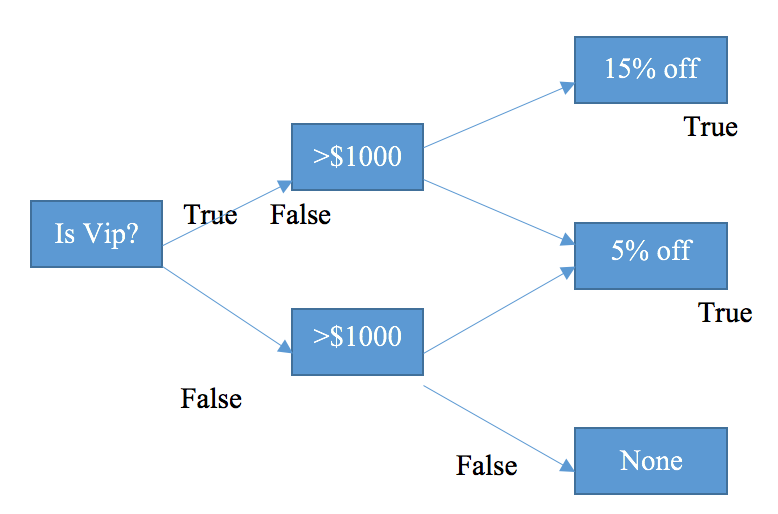
\includegraphics[width=8.0cm]{ctree.png} 
\newline
\caption{An Example of C4.5 Decision Tree}
\label{fig:ctree} 
\end{figure}

We adopt C4.5 to generate a decision tree for the problem. The algorithm is proposed by Ross Quinlan~\cite{Quinlan}, which is an extension of his earlier ID3 algorithm.
The pseudocode~\cite{Kotsiantis} of the general algorithm for building decision trees by C4.5 is: 

\begin{enumerate}
\item Check for base cases.
\item For each attribute a, find the normalized information gain ratio from splitting on a.
\item Let a\_best be the attribute with the highest normalized information gain.
\item Create a decision node that splits on a\_best.
\item Recur on the sublists obtained by splitting on a\_best, and add those nodes as the children of the node.
\end{enumerate}

\section{Results}
\subsection{Data Sets}
All the data come from Dotabuff, which is the largest third-party Dota2 game track website. In the team section of Dotabuff, there are more than 1,000 teams sharing their game results. We write a crawler to collect our data by Python urllib2 and Beautifulsoup libraries. As Section II mentioned, to keep the balance of the data set, for one game, we generate two feature vectors. We will first generate one vector based on the original information provided in the website. Then we will swap the features of two teams to generate the second vector. We kept running the crawler for four days to collect data.
Our data sets include 15,197 Dota2 matches records from top 100 famous teams in the world. Each row has 423 features including team ID, hero lineup and result.

\subsection{Training and Testing}
We use 10-fold cross-validation as our training and testing methods. The original data sets are randomly partitioned into 10 equal sized subsets, use one of the subsets as the test set and the others as the testing set. The process is to repeate 10 folds, with each subset used exactly once as the testing set. The results are the combined from 10 folds.

\subsection{Evaluation Metrics}
F-score is used as the evaluation metric our experiment, since both the precision and recall are considered by this method. F-score can be calculated by the following formulas.

\begin{equation}
F=2\times\frac{Precision+Recall}{Precision*Recall}
\end{equation}

\begin{equation}
Precision = \frac{\#TruePositives}{\#TruePositives+\#FalsePositives}
\end{equation}

\begin{equation}
Recall = \frac{\#TruePositives}{\#TruePositives+\#FalseNegatives}
\end{equation}

We also use Confusion Matrix to present our results. A sample form is described in Table~\ref{table:sample}. There are 200 samples in the testing data set. 200 instances are classified correctly, and 100 instances are classified wrongly.

\begin{table}
\begin{center}
\begin{tabular}{|c|c|c|}
\hline
Predicted: True & Predicted: False & N = 200 \\ \hline
100 & 50 & Actual: True \\ \hline
50 & 100 & Actual: False \\ \hline
\end{tabular}
\caption{A Sample of Confusion Matrix}
\label{table:sample}
\end{center}
\end{table}

\subsection{Results}
Due to 10-fold cross-validation, every instance in the data sets has been used as test cases. There are 15,197 samples in all. 9,247 instances (60.8475\%) have been classified correctly, and 5,950 instances (39.1525\%) have been classified incorrectly. The accuracy by class and confusion matrix can be seen in Table~\ref{table:accuracy} and Table~\ref{table:matrix}.

\begin{table}
\begin{center}
\begin{tabular}{|c|c|c|c|}
\hline
Class & Precision & Recall & F-score \\ \hline
0 & 0.609 & 0.608 & 0.654 \\ \hline
1 & 0.608 & 0.609 & 0.654 \\ \hline
\end{tabular}
\caption{Detailed Accuracy by Class}
\label{table:accuracy}
\end{center}
\end{table}

\begin{table}
\begin{center}
\begin{tabular}{|c|c|c|}
\hline
a & b & \\ \hline
4,620 & 2,978 & a = 0 \\ \hline
2,972 & 4,627 & b = 1 \\ \hline
\end{tabular}
\caption{Confusion Matrix}
\label{table:matrix}
\end{center}
\end{table}

\subsection{Results from Other Models}
We also applied other models to the problem. The results are shown in Table~\ref{table:others}

\begin{table}
\begin{center}
\begin{tabular}{|c|c|}
\hline
Model & F-score \\ \hline
Logistic Regression & 54.08\% \\ \hline
Natural Network & 59.51\% \\ \hline
Support Vector Machine & 60.43\% \\ \hline
Native Bayes & 58.92\% \\ \hline
\end{tabular}
\caption{Results from Other Models}
\label{table:others}
\end{center}
\end{table}

\section{Related Work}
XXX: Add several papers

\section{Conclusion}

This paper proposes a method to predict the ESports game result of Dota/Dota2. With three-type features (Team ID, Hero Lineup and Result) and decision tree model, our Dota/Dota2 prediction system gets 65.4\% F-score from a data set of 15,197 matches. 
The F-score is not relatively high and the reasons are as follows:
\begin{enumerate}
\item Concerning the data sets, we can only get the game records including the information of Team ID, Hero Lineup and result. More detailed information about teams and games are not available.
\item Regarding features, player’s skills, physical and emotional condition and the external environment all are vital to the result of a game, but none of them can be measured.
\end{enumerate}

% References should be produced using the bibtex program from suitable
% BiBTeX files (here: strings, refs, manuals). The IEEEbib.bst bibliography
% style file from IEEE produces unsorted bibliography list.
% -------------------------------------------------------------------------
\vfill\pagebreak

\bibliographystyle{abbrv}
\bibliography{./Template}

\end{document}
